\newcommand{\code}{\texttt}
\renewcommand\theadalign{bc}
\renewcommand\theadfont{\bfseries}
\renewcommand\theadgape{\Gape[4pt]}
\renewcommand\cellgape{\Gape[4pt]}

\chapter{The project}
\section{Anomaly detection in network traffic}
System administrators often need to quickly identify causes behind anomalous network traffic. This however can be very difficult to do manually,
and for this reason network analysis tools are used in order to easier identify causes behind anomalous behaviour. This project attempts to replicate
a recently published method of network anomaly detection for \emph{ICS} (Industrial Control System) traffic \cite{burgetova_anomaly}.

ICS communication is generally well protected against external threats of cyberattacks, however as soon as an endpoint is compromised,
the attack prevention mechanisms begin to fail \cite{burgetova_anomaly}. ICS traffic is generally highly stable in packet exchange frequency and
intermediate node count, and therefore can be subject to statistical modeling based on these features.
As an attacker may initiate various attacks from the compromised node, particularly by tampering with packet counts, a model of normal traffic communication
may be used to discriminate the anomalous traffic.


\section{Standard IEC 60870-5-104}
The IEC 60870 set of standards define systems used for telecontrol in electrical engineering and power system automation applications,
part 5 of which provides a communication profile for sending basic telecontrol messages between a central telecontrol station and telecontrol outstations.
This communication profile uses permanent and directly connected data circuits \cite{IEC104}. Part 5 of these standards consists of multiple
additional parts and this project focuses on parts 101 and its extension, 104 (further as IEC 104).

\subsection{Packet structure}
The IEC 104 packets are encapsulated within TCP/IP packets providing reliable delivery. Every IEC 104 packet
contains an \emph{APDU} (Application Protocol Data Unit), which encapsulates two other sections.
An \emph{APCI} (Application Protocol Control Information) section of a fixed length of 6 bytes and a variable length \emph{ASDU} section.

Each APCI starts with a 0x68 byte followed by an 8-bit value of the length of the APDU (this length does not include the first two bytes of the APCI).
The final four bytes of the APCI are 8-bit control fields. The two least significant bits of the first control field signify the type of the telecontrol message.
The type may be one of three formats - I, S or U and only the I format contains an ASDU. An APDU always contains an APCI.
The ASDU is a variable length data structure, consisting of two sections. A \emph{DUI} (Data Unit Identifier) section with a fixed length of 6 bytes and
a variable length data section \cite{mai2019iec}\cite{IEC104}. An illustraction of the packet structure can be seen in figure \ref{fig:packet_structure}.

\begin{figure}
  \centering
  \begin{subfigure}[b]{0.3\textwidth}
    \centering
    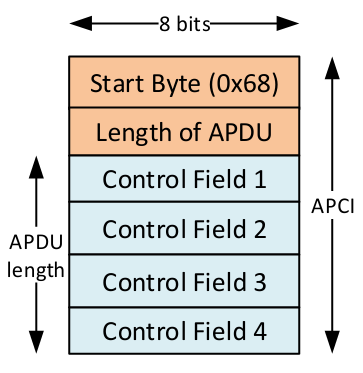
\includegraphics[width=\textwidth]{obrazky-figures/apdu_fixed_length.png}
    \caption{fixed length APDU}
    \label{fig:fixed_length_APDU}
  \end{subfigure}
  \hfill
  \begin{subfigure}[b]{0.3\textwidth}
    \centering
    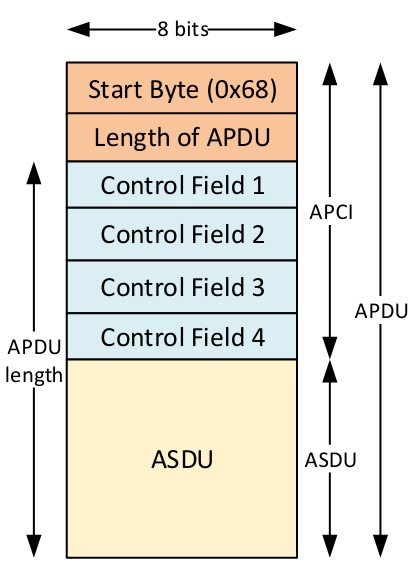
\includegraphics[width=\textwidth]{obrazky-figures/apdu_variable_length.png}
    \caption{variable length APDU}
    \label{fig:variable_length_APDU}
  \end{subfigure}
  \hfill
  \begin{subfigure}[b]{0.3\textwidth}
    \centering
    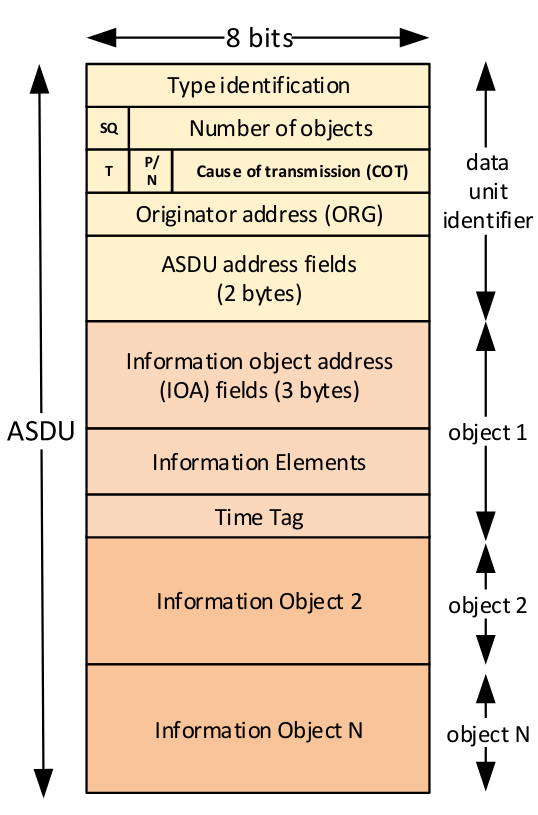
\includegraphics[width=\textwidth]{obrazky-figures/asdu.png}
    \caption{ASDU}
    \label{fig:ASDU}
  \end{subfigure}
  \caption{Visualization of the APCI and ASDU fields. Taken from \cite{IEC104}.}
  \label{fig:packet_structure}
\end{figure}

\section{The dataset and statistical modeling}
For this project the \code{mega104-17-12-18} dataset was used. The raw dataset contains over $150000$ packets captured over the course of
about $68$ hours. However, as we are only interested in IEC 104 communication, the irrelevant packets have been filtered out, which left us
with $58929$ IEC 104 packets in total. The dataset contains one master and one slave endpoint.

As described in \cite{burgetova_anomaly}, the inter arrival times of subsequent packets can be used for statistical modeling of
IEC 104 communication. These are acquired through the subtraction of arrival times of individual consecutive packets. The utilized pcap dataset contains metadata
with these packet arrival times, and therefore could be used for modeling. The direction of the packets can be classified by either the source and destination IP
addresses, or by the source and destination transport layer ports.
%// TODO dont know if this is correct: The specific classification of master-to-slave or slave-to-master directions is not
%important in the method put forward in \cite{burgetova_anomaly}, as the resulting statistical model does not differentiate between the two.

\subsection{Anomaly detection method}
The anomaly detection method used is the same as in \cite{burgetova_anomaly}. It utilizes the inter-arrival times of consecutive packets to build a
statistical model capable of detecting various anomalies in the network.
First the input dataset is split into two directions - communication from master to slave and from slave to master. This is done because the opposing
directions have different communication characteristics. The timing metadata is gathered and time differences for each direction are computed, such that
$\Delta t_{i} = \Delta t_{i+1} - \Delta t_{i}$. The result is a list of $\Delta t$ values of inter arrival times (this list will bereferred to as $\Delta T$).

\subsubsection{Split-points}
The used anomaly detection method hinges on the concept of a split-point. The split-point defines a suitable value in the range of
observed $\Delta t$ values. Its function is to split the $\Delta T$ list into two new lists - one, where $\Delta t < split\text{-}point$ and another,
where $\Delta t \geq split\text{-}point$. Before choosing a suitable split-point, four initial values per direction are computed - the $Q1$, $Q2$, $Q3$ quartiles
and the mean of $\Delta T$. The candidate split-points should be computed for any communication dataset individually, as the communication between various
devices has different characteristics, making it infeasable to use fixed split-point candidates. The $\Delta T$ list is to be split by each candidate
split-point as stated above.

\subsubsection{Time windows}
All of the gathered data based on the candidate split-points now needs to be grouped together into 5-minute windows based on the original packet
timestamps. The sizes of these windows are then computed (i.e. the number of packets per each 5 minute window). These window sizes are subsequently used to
choose the most suitable split-point for the dataset. The chosen split-point is the one that generated window sizes with the lowest standard deviation,
and which conforms to the condition $(mean(window\text{ }sizes) - 3*std(window\text{ }sizes)) > 0 $. The calculated standard deviation and mean belonging
to the chosen split-point is saved. Time window distributions for the from-master direction with split-point $8.0006$ and for the to-master direction
with split-point $11.1537$ are shown in figure \ref{fig:window_size_graphs}.

\subsubsection{The final profile}
The final profile is a 4-tuple of the following form:\\
$(split\text{-}point, \left\langle all^{-}, all^{+} \right\rangle,
\left\langle lt^{-}, lt^{+} \right\rangle, \left\langle geq^{-}, geq^{+} \right\rangle)$, where $split\text{-}point$ is the most suitable split-point,
and the three ranges denote the valid number of packets for any 5 minute window according to the three-sigma-rule, such that $all$ applies to the number of all packets
within a window, $lt$ applies to the number of packets with $\Delta t$ less than the split-point, and $geq$ applies to the the number of packets with $\Delta t$
greater or equal to the split-point. The three sigma rule defines the interval $\left\langle mean - 3\sigma , mean + 3\sigma \right\rangle$.

\begin{figure}
  \centering
  \begin{subfigure}[b]{0.49\textwidth}
    \centering
    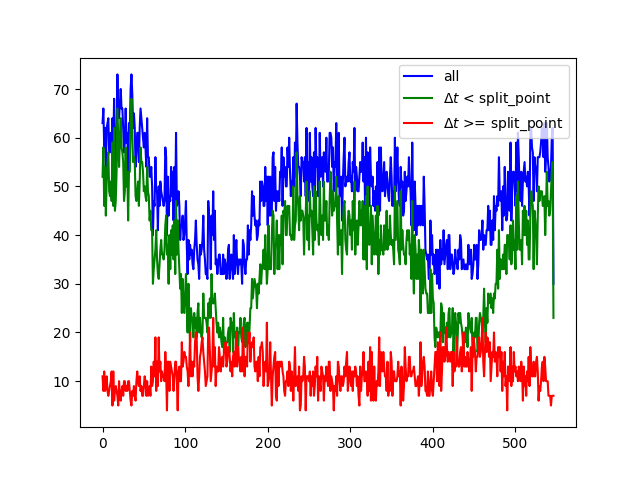
\includegraphics[width=\textwidth]{obrazky-figures/from_master.png}
    \caption{from master}
    \label{fig:master_slave}
  \end{subfigure}
  \hfill
  \begin{subfigure}[b]{0.49\textwidth}
    \centering
    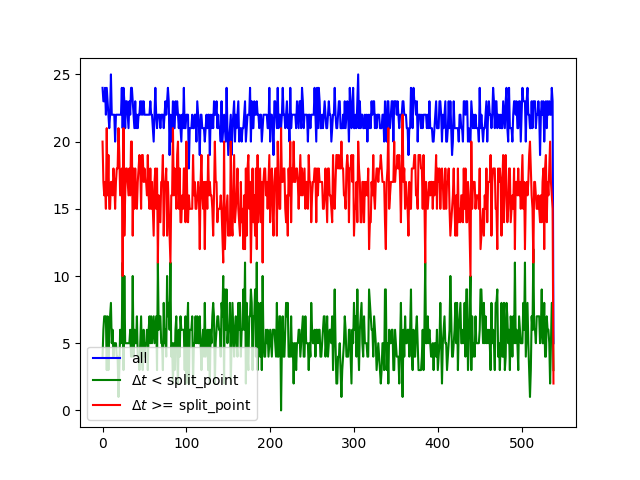
\includegraphics[width=\textwidth]{obrazky-figures/to_master.png}
    \caption{to master}
    \label{fig:slave_master}
  \end{subfigure}
  \caption{Window sizes in directions from and to master.}
  \label{fig:window_size_graphs}
\end{figure}

\section{Evaluation and conclusion}
The profile was built from two thirds of the provided dataset \code{mega104-17-12-18} and validated on the final third of the dataset. Table
\ref{tab:validation} shows the validation results for simple anomaly detection, where each time window outside the expected range is counted as
an anomaly.
In conclusion, we were able to partially reproduce the results of \cite{burgetova_anomaly}.

\begin{table}
  \centering
  \caption{Validation results for dataset \code{mega104-17-12-18}.}
  \begin{tabular}{| l | r | c | c |}
    \hline
    \thead{Direction} & \thead{Split\\category} & \thead{False\\Positives} & \thead{Accuracy} \\
    \hline
    \multirow{3}{1em}{from master} & $all$ & $1/277$ & $99.6390\%$ \\
      & $< split\text{-}point$ & $0/277$ & $100\%$ \\
      & $\geq split\text{-}point$ & $0/277$ & $100\%$ \\
    \hline
    \multirow{3}{1em}{to master} & $all$ & $1/269$ & $99.6283\%$ \\
      & $< split\text{-}point$ & $0/269$ & $100\%$ \\
      & $\geq split\text{-}point$ & $4/269$ & $98.5130\%$ \\
    \hline
  \end{tabular}
\end{table}\label{tab:validation}


